\documentclass[a4paper,10pt,oneside]{article}
\usepackage{graphicx}
\usepackage{color}
\usepackage{url}
\usepackage{subfigure}
\usepackage[utf8]{inputenc}
\usepackage[T1]{fontenc}
\usepackage{tgpagella}
%\usepackage[scale=0.9]{tgcursor}
%\usepackage[scale=0.9]{tgheros}

\newcommand{\myscale}{0.74}
\newcommand{\vect}[1]{\boldsymbol{#1}}
\newcommand{\code}[1]{\texttt{#1}}
\newcommand{\jmodule}[1]{\texttt{\textsl{#1}}}

\setlength{\hoffset}{-1in} %left margin will be 0, as hoffset is by default 1inch
\setlength{\voffset}{-1in} %analogous voffset
\setlength{\oddsidemargin}{1.5cm}
\setlength{\evensidemargin}{1.5cm}
\setlength{\topmargin}{1.5cm}
\setlength{\textheight}{24cm}
\setlength{\textwidth}{18cm}

\def\mftitle{jInfer TwoStep simplifier design and implementation}
\def\mfauthor{Michal Klempa, Mário Mikula, Robert Smetana, Michal Švirec, Matej Vitásek}
\def\mfadvisor{RNDr. Irena Mlýnková, Ph.D., Martin Nečaský, Ph.D.}
\def\mfplacedate{Praha, 2011}
\title{\bf\mftitle}
\author{\mfauthor \\ Advisors: \mfadvisor}
\date{\mfplacedate}

\ifx\pdfoutput\undefined\relax\else\pdfinfo{ /Title (\mftitle) /Author (\mfauthor) /Creator (PDFLaTeX) } \fi

\begin{document}
\maketitle
\noindent Target audience: developers willing to extend jInfer, scientist willing to implement own inference methods

\noindent \emph{Note: we use the term \textbf{inference} for the act of creation of schema throughout this and other jInfer documents.}

\section{Using of factory pattern}
\begin{figure}
	\centering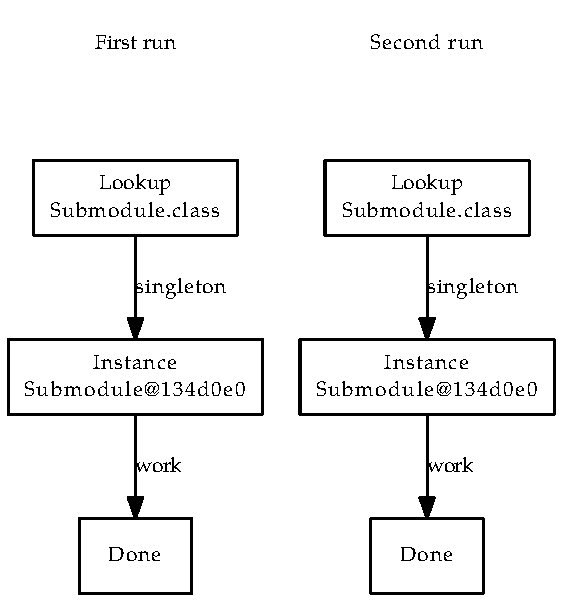
\includegraphics[scale=\myscale]{factory_pattern1}
	\caption{Same instance of class returned by NetBeans in two successive inference runs} \label{factory_pattern1}
\end{figure}
\jmodule{TwoStepSimplifier} is divided into three submodules, which are then divided into submodules and so on.
Each submodule is simply class, properly anotated.
User selects proper classes - submodules to work in chain on inference.
Classes are then, in runtime looked up by using NetBeans lookup mechanism (see \cite[p. 16]{arch}).
But NetBeans holds one instance of each class, that may be looked upon.
When user runs inference first time, classes are looked up and used.
Maybe class members are initialised, instances are in some state after inference completes.
Then, user clicks run button again, and same instances of classes are returned by lookups.
Oops, theese are not freshly created instances, using them as they are may cause harm.
The problem is ilustrated on fig. \ref{factory_pattern1}.
\begin{figure}
	\centering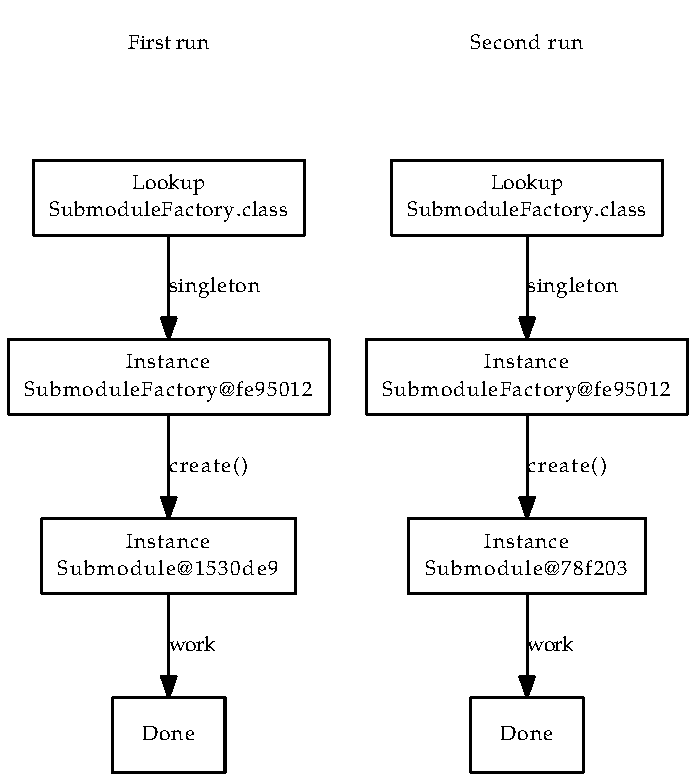
\includegraphics[scale=\myscale]{factory_pattern2}
	\caption{Factory solution of singleton lookup class problem} \label{factory_pattern2}
\end{figure}

There are basically two solutions:
\begin{itemize}
	\item force each class (submodule) that is being looked up in inference process, to implement
some sort of cleanup method, that would restart it into fresh state and make it ready to use by another 
inference run,
	\item or create new instances of theese classes in each inference run and make singleton classes (those which NetBeans return by lookups) their factory classes.
\end{itemize}
We decided for the latter approach (as ilustrated on fig. \ref{factory_pattern2}
It enables us not only to produce fresh class instance in each inference run, but also factory classes implement obligatory
module methods such as \code{getName}, \code{getDescription} and so on, which are really same in each inference run.
Each submodule is then defined by (at least) two interfaces.
One is the factory interface, like this one:
\begin{verbatim}
public interface AutomatonSimplifierFactory extends 
                     NamedModule, Capabilities, UserModuleDescription {
  <T> AutomatonSimplifier<T> create();
}
\end{verbatim}
It extends \code{NamedModule} with its modules describing methods:
\begin{verbatim}
String getName();
String getDisplayName();
String getModuleDescription();
\end{verbatim}
It extends \code{Capabilities}, thus each module have to answer, if it has some capabilities.
And, in TwoStep we often extend \code{UserModuleDescription}, which defines method:
\begin{verbatim}
String getUserModuleDescription();
\end{verbatim}
It returns description of the module, comprehensive to user, which is then displayed in properties panels.

In some circumstances, it is useful to have method \code{create()} generic.
The \jmodule{AutomatonSimplifier} works with \code{Automaton}, which itself is generic too.
But simplifying does not depend on type of symbol of automaton, so interface \code{AutomatonSimplifier<T>}
is also generic as simplifier can simplify automaton of any java type symbol.
Factory interface deals with this by defining \code{create()} method generic too.

Second interface is the one, which is returned by \code{create()} method.
That is the interface, which defines real work cycle with submodule (in example it is \code{AutomatonSimplifier<T>}).
We call this interface the worker interface of submodule.
Usage of this factory pattern follows the routine:
\begin{verbatim}
final Properties p = RunningProject.getActiveProjectProps(getName());

AutomatonSimplifierFactory f = ModuleSelectionHelper.lookupImpl(AutomatonSimplifierFactory.class,
   p.getProperty(PROPERTIES_AUTOMATON_SIMPLIFIER));

AutomatonSimplifier<AbstractStructuralNode> autSmp = f.<AbstractStructuralNode>create();
...
give some work to autSmp
\end{verbatim}
If our module has some submodules, we often implement lookups for submodules implementations in our own factory create method.
Worker class receives factories of all submodules it needs as a constructor parameters.

Lets look on \code{AutomatonMergingStateFactory}, that is factory of module, which has AutomatonSimplifier as submodule.
Its create method looks like this (shortened): 
\begin{verbatim}
@Override
public ClusterProcessor<AbstractStructuralNode> create() {
  LOG.debug("Creating new ClusterProcessorAutomatonMergingState.");
  return new AutomatonMergingState(getAutomatonSimplifierFactory(), getRegexpAutomatonSimplifierFactory());
}
\end{verbatim}
Methods \code{getAutomatonSimplifierFactory} and \code{getRegexpAutomatonSimplifierFactory} are analogical, we show you the former one:
\begin{verbatim}
private AutomatonSimplifierFactory getAutomatonSimplifierFactory() {
  final Properties p = RunningProject.getActiveProjectProps(getName());

  return ModuleSelectionHelper.lookupImpl(AutomatonSimplifierFactory.class,
            p.getProperty(PROPERTIES_AUTOMATON_SIMPLIFIER));
}
\end{verbatim}
Cluster processor \code{AutomatonMergingState} then receives factories of \code{AutomatonSimplifier} and \code{RegexpAutomatonSimplifier} submodules in its constructor.
Cluster processor then may create as many instances of submodule classes as it needs (maybe simplifying more than one automaton).
Thorough this document, we will mention only worker interface when describing submodules, since all factory interfaces are designed same way just described.

\section{TwoStep module}
TwoStep simplifier is inspired by \cite{1802522} design. Inference proceeds in two steps:
\begin{enumerate}
	\item clustering of element instances into clusters of (probably) same elements
	\item infering regular expression for each element from examples of element contents taken from all elements in cluster
\end{enumerate}
Main routine of TwoStep simplifer does basically this:
\begin{verbatim}
// 1. cluster elements
final Clusterer<AbstractStructuralNode> clusterer= clustererFactory.create();
clusterer.addAll(initialGrammar);
clusterer.cluster();

// 2. prepare emtpy final grammar
final List<Element> finalGrammar= new LinkedList<Element>();

// 3. process rules
final ClusterProcessor<AbstractStructuralNode> processor= clusterProcessorFactory.create();
for (Cluster<AbstractStructuralNode> cluster : clusterer.getClusters()) {
  final AbstractStructuralNode node =  processor.processCluster(clusterer, cluster.getMembers() - without sentinels);
  // 4. add to rules
  finalGrammar.add(new Element(node.getContext(),
                   node.getName(),
                   node.getMetadata(),
                   ((Element) node).getSubnodes(),
                   attList);
}
\end{verbatim}
Task of clustering is dedicated to \jmodule{Clusterer} submodule, and task of infering regular expression for each cluster is dedicated to \jmodule{ClusterProcessor} submodule. We will examine both of them.
There is also third submodule called \jmodule{RegularExpressionCleaner} actually, its purpose is just to beatify output regular expressions, no inference logic is implemented there. 
Modules currently in jInfer are drawn on fig. \ref{twostep_modules}.
\begin{figure}
	\centering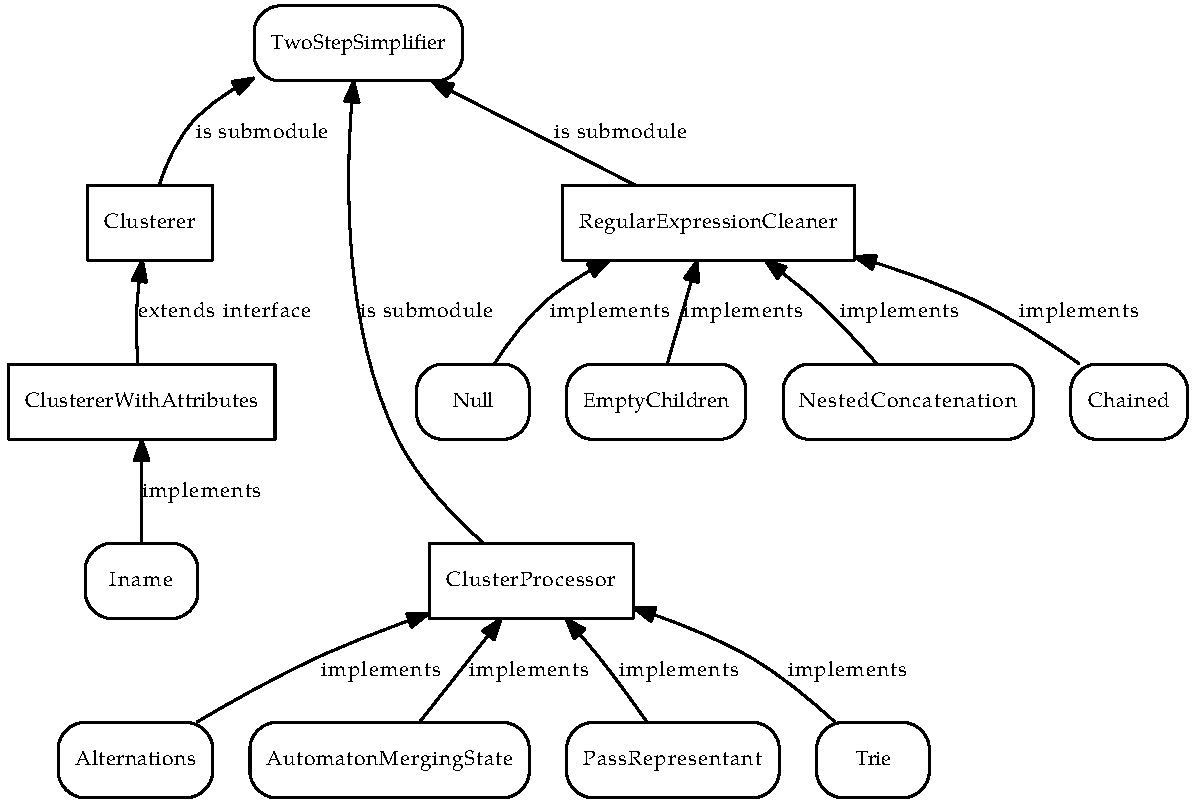
\includegraphics[scale=\myscale]{twostep_modules}
	\caption{Submodules of TwoStep simplifier} \label{twostep_modules}
\end{figure}
We provide one \jmodule{Clusterer} and four \jmodule{ClusterProcessor} implementations.
Each of those will be explained further in this document.

TODO sentinel processing

\subsection{Clusterer submodule}
Lets start by example, let input document(s) contain XML:
\begin{verbatim}
<person name="john" surname="smith">
  <info>
   Some text
   <note/>
  </info>
</person>
<inform>
  Another text
  <note/>
</inform>
<person>
    <information>
      Some text
      <note/>
    </information>
</person>
\end{verbatim}
We examine info-like named elements.
If we cluster elements sipmly by their name, we get one cluster with info element, another cluster with inform element and another one with information element.
As \cite{1802522} suggests, we should consider element content in clustering process.
If we take care of element content, elements info, inform and information would look same (in means of node tree inside them - text node and element note).
Elements information and info have even same context (inside person element).

We implement clustering in \code{cz.cuni.mff.ksi.jinfer.twostep.clustering} package.
One cluster is represented by class \code{Cluster<T>} with \code{T} as type of clustered items.
This class simply holds java set of member of cluster and one of the references is held also in \code{representant} member.

We provide \code{Clusterer} interface for classes to implement.
Its purpose is to cluster bunch of elements (rules) on input, into  bunch of cluster class instances (cluters) on output.
It has methods \code{add()} and \code{addAll()} for adding items for clustering.
Center is method \code{cluster()}, which does the clustering itself.
As it may be time-consuming operation, method throws \code{InterruptedException}.
Implementation should take care of checking whether thread is user interrupted (see \cite[p. 12]{arch}).
After clustering, implementation should hold clusters in member, as it it will be further asked by calling method \code{T getRepresentantForItem(T item)}.
Given item to this method, one can ask for representant of cluster, to which the item belongs.
If no such cluster exists (item was not added for clustering before), we recommend you throwing an exception rather than returning \code{null}.
Missing item will probably  indicate error in algorithm rather than normal workflow.
One can pull clusters from clusterer by calling \code{getClusters()} method.

Basic work usage of clusterer is:
\begin{verbatim}
Clusterer <T> c = new MyContextClusterer<T>();
c.addAll(initialGrammar);
c.cluster();
...
c.getClusters();
or
c.getRepresentantForItem(x);
\end{verbatim}

\subsubsection{ClustererWithAttributes extended interface}
Maybe you noticed that whole clusterer interface and cluster class are generic.
They may be used as design pattern not only for clustering elements in inference process.
To address clustering of elements in more detail, we created \code{ClustererWithAttributes<T, S>} interface, which extends \code{Clusterer<T>} interface.
It adds method \code{List<Cluster<S>{}> getAttributeClusters(T representant)}, implying that each representant of
type \code{T} (that is representant of some main cluster) has some "attribute" clusters associated with it.
Attribute clusters are of type \code{S} and can be retrieved by calling \code{getAttributeClusters(x)}.


Finally, we use this scheme to implement clusterer \code{Iname<AbstractStructuralNode, Attribute>} class, which takes \code{AbstractStructuralNode} classes to cluster as main, and \code{Attribute} classes as attributes.
For each cluster of elements, it creates list of clusters of attributes observed with all elements in main cluster.

All simple data are considered equal and given one dedicated cluster.
But in future implementations, extensibility is ensured to cluster simple data to obtain content models of elements.

All sentinel elements are clustered too.
TODO sentinels
TODO attributes clustering

\subsection{ClusterProcessor submodule}
Cluster processor takes rules of one cluster of element and somehow obtains regular expression for that set of elements. It returns rule - element with name set to desired name of element in schema (not all elements in cluster have to have same name, if advanced clustering scheme is used, then processor has to choose right name for  resulting element) and with subnodes set to regular expression infered.
It process attributes of all elements in cluster to obtain meaningful schema attribute specification and theese attributes has to attach to resulting element.

Worker interface itself is defined as follows:
\begin{verbatim}
public interface ClusterProcessor<T> {
  T processCluster(
          final Clusterer<T> clusterer,
          final List<T> rules
          ) throws InterruptedException;
}
\end{verbatim}
Maybe you are asking, why cluster processor is given the clusterer instance.
Rules themself contain information about which elements to process, but clusterer has more information
about the topic.
Clusterer can tell you representant for any element in whole input (not only those elements in rules, but also those that may be on right side of rules), clusterer (if it is with attributes) has information about attributes <of each cluster.

We will now shortly describe each cluster processor implementation we've got.

\subsubsection{PassRepresentant}
Simple example to read. For each cluster return its representant as a rule to be in schema.
This has nothing to do with infering grammar, it is just proof of submodules concept.
Input documents are not valid against this odd grammar.
Do not use this in practice, just read the code to understand the bare minimum needed to implement submodule.

\subsubsection{Alternations}
This processor simply gets all right sides from elements in cluster, puts them in one big list and creates alternation regular expression with this list as children.
That is, it creates one big rule with alternation of every positive example observed.
No generalization is done at all.

\subsubsection{Trie}
This processor takes all rules in a cluster, treats them like strings and builds a prefix tree (a ``trie") of them. More precisely, it takes the first rule and delares it to be a long branch (concatenation of tokens) in a newly created tree. After that, it adds the remaining rules one by one as branches like this: as long as it can follow an existing branch, it follows it. As soon as the newly added branch starts to differ, it ``branches off" (creates an alternation at that point) the existing tree and hangs the rest of the newly added rule there. Repeating this process creates a prefix tree describing all the rules in the cluster.

\subsubsection{AutomatonMergingState}
AutomatonMergingState is implementation of merging state algorithm on nondeterministic finite automaton.
It creates prefix-tree automaton (PTA) from positive examples - right sides of rules given.
Then it calls its submodule called \jmodule{AutomatonSimplifier} to  modify PTA to some generalized 
automaton by merging states.

Simplified automaton is then converted to an instance of \code{RegexpAutomaton} by using clone constructor in regexp automaton.
Regexp automaton is automaton with regular expression as symbol on transitions.
In automata theory, such automaton is called extended NFA.
Clone constructing is done by converting each symbol in source automaton to regexp token with that symbol as content.

Regexp automaton is then passed into second submodule called \jmodule{RegexpAutomatonSimplifier}.
Its job is to derive regular expression from automaton, such that automaton and regular expression represents same language.

AutomatonMergingState has one more submodule, the \jmodule{MergeConditionTester}, which is not called directly by AutomatonMergingState.
It is at disposal for implementations of AutomatonSimplifier interface for testing, whether two states in automaton are equivalent and should be merged into one state.

AutomatonSimplifier implements solution searching logic in simplifying automaton by merging states.
We implement greedy strategy in class \code{Greedy}.
It simply asks given MergeConditionTester if it can merge any of automaton states and merges states until there are no states to be merged (on every pair of states asked, MergeConditionTester answers, they cannot be merged).
One can implement ACO heuristics or MDL principle heuristics as AutomatonSimplifier submodule using MergeConditionTesters provided.

Whole submodule structure of AutomatonMergingState cluster processor is drawn on fig. \ref{automaton_merging_state_modules}.
\begin{figure}
	\centering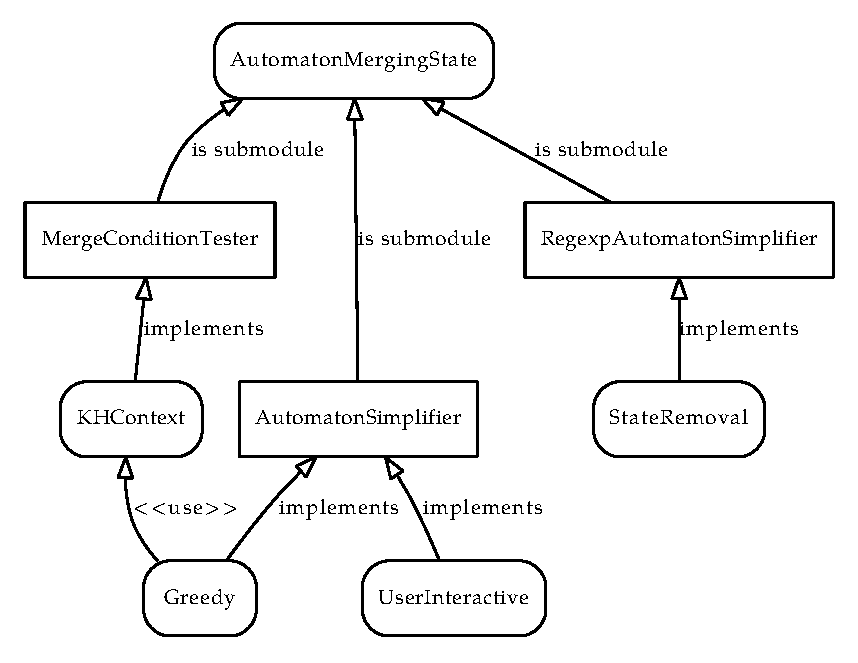
\includegraphics[scale=\myscale]{automaton_merging_state_modules}
	\caption{Submodules of AutomatonMergingState cluster processor} \label{automaton_merging_state_modules}
\end{figure}
We have implemented \emph{k,h-context} (see \cite{ahonen}) state equivalence in class \code{KHContext}, which is used by \code{Greedy}
to test mergability of states by default configuration.

\subsubsection{StateRemoval}
\begin{figure}
	\centering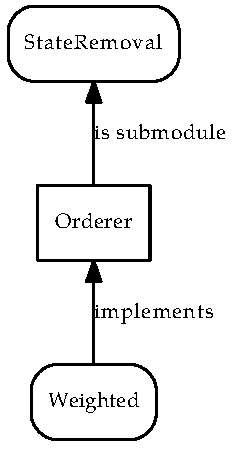
\includegraphics[scale=\myscale]{state_removal_modules}
	\caption{Modules of StateRemoval.} \label{state_removal_modules}
\end{figure}
We are using state removal method (see \cite{1224321}) to convert regexp automaton into equivalent regular expression.
This is implemented in \code{StateRemoval} class (on fig. \ref{state_removal_modules}).
We defined one submodule of this class with interface called \code{Orderer}.
It has only one method to implement: \code{getStateToRemove}.
Given automaton it has to return reference to one state which should be removed from automaton at first.
State removal calls this submodule and removes states given until there are only two states in automaton - superInitial and superFinal states,
with exactly one transition.
That transition has final regular expression on it as symbol, it is read and returned to AutomatonMergingState.
We implement one orderer, called \code{Weighted}.
It is simple heuristic - weights all states (weight = sum of {in | out | loop}-transition regular expression lengths) and returns state with lowest weight.

\subsection{RegularExpressionCleaner module}
Last we examine \code{RegularExpressionCleaner} interface.
TODO anti cleaners

Whole TwoStep submodules structure is on fig. \ref{twostep_modules_complete}.
\begin{figure}
	\centering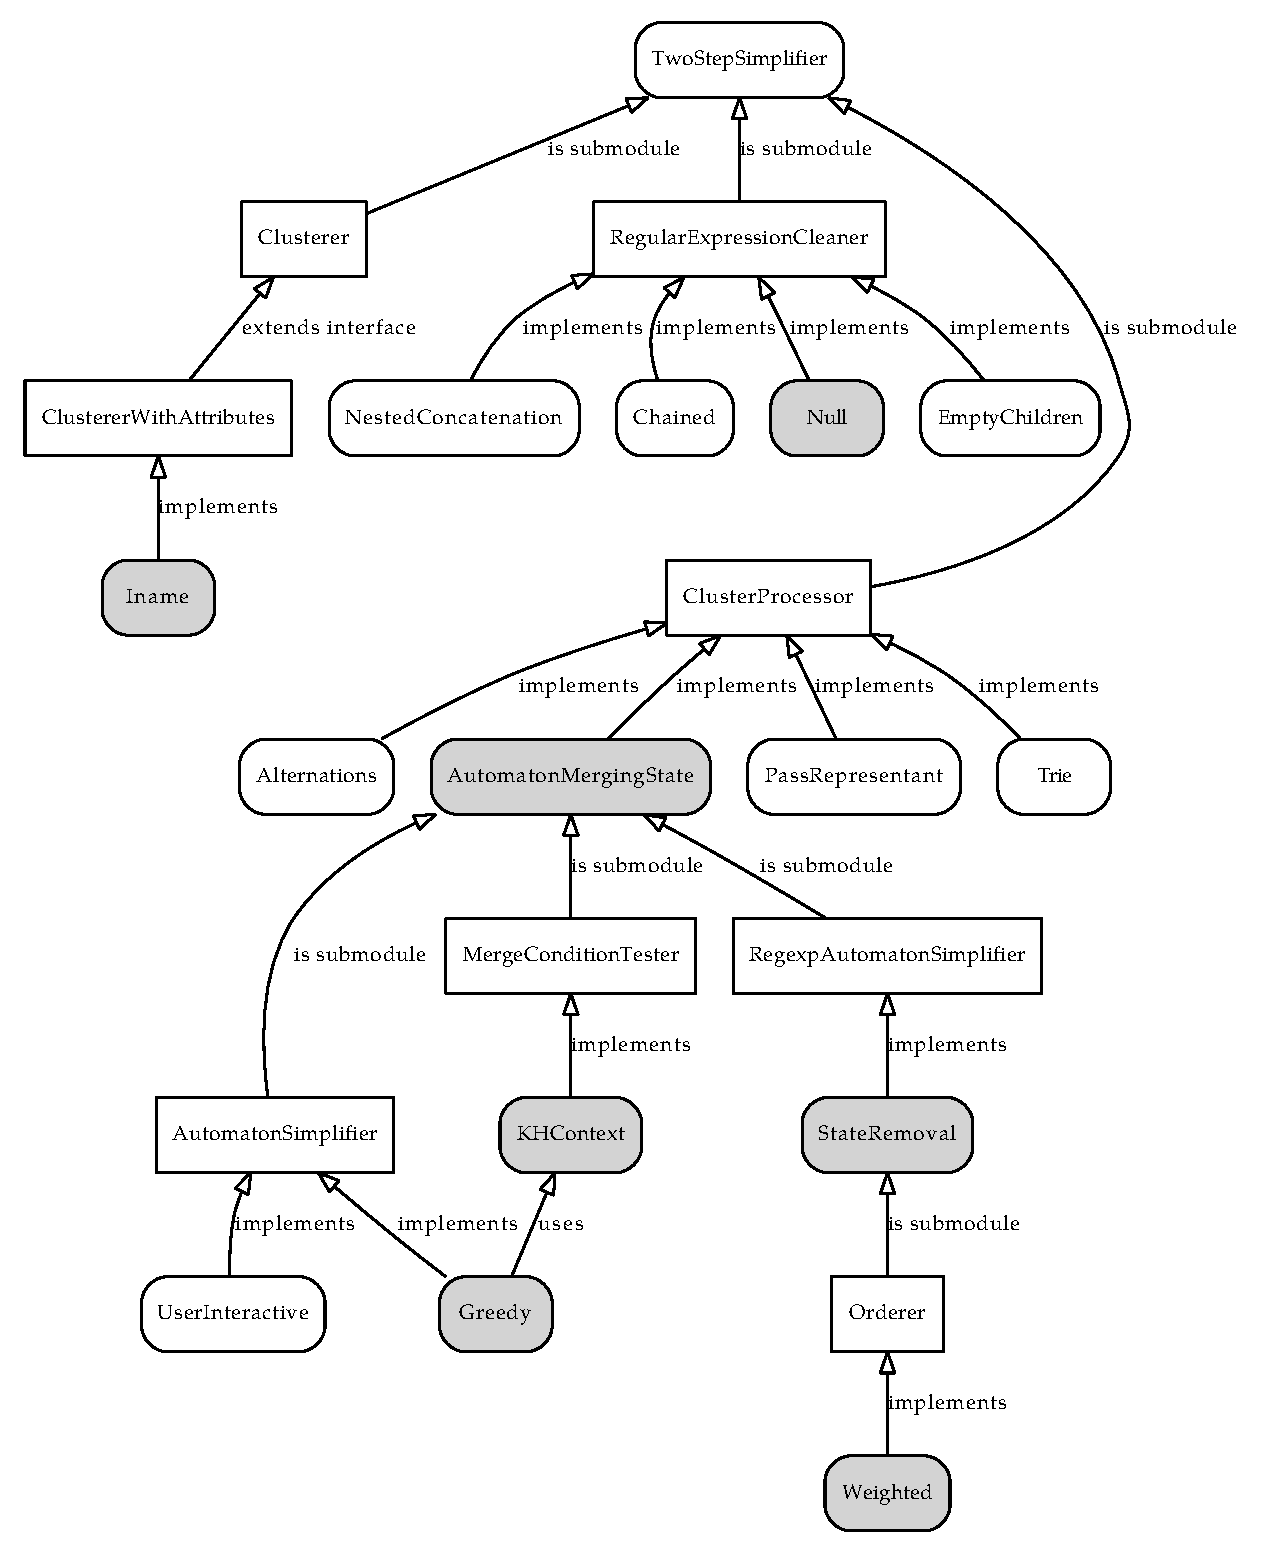
\includegraphics[scale=\myscale]{twostep_modules_complete}
	\caption{Modules of TwoStep simplifier and their submodules. Filled classes are default selection (best of).} \label{twostep_modules_complete}
\end{figure}

\nocite{*}
\bibliographystyle{alpha}
\bibliography{literature}

\end{document}
